\section{Interest Flooding Attacks in NDN}
\label{sec:interest flooding}

% Points here:
% - Classification
% - Mechanisms: congestion and memory exhaustion
% - Target
% - Effectiveness: random names, non-existing content
% - Assumptions: the network, attackers, attack traffic, and legitimate consumers

%??? - References to the discussion about other types of attacks (ordifferent attack assumptions) about other attacks and explicitly stating that this work aims to build a baseline for general Interest Flooding mitigation problem, with other attack profiles and malicious gateways.

\paragraph{What is it?}

Unlike data packets, Interest packets in NDN are unsolicited, consume state in intervening routers and are routed based on content name prefixes in the network. Such properties makes Interest packets an effective tool in launching DoS attacks in NDN. An attacker or a set of distributed attackers can inject excessive amounts of Interests to overload the network and cause service disruptions for legitimate users (Fig.~\ref{fig:flooding example}). We coin in the term \emph{Interest flooding} to refer to these network-level flooding attacks.

\begin{figure}[htbp]
  \centering
  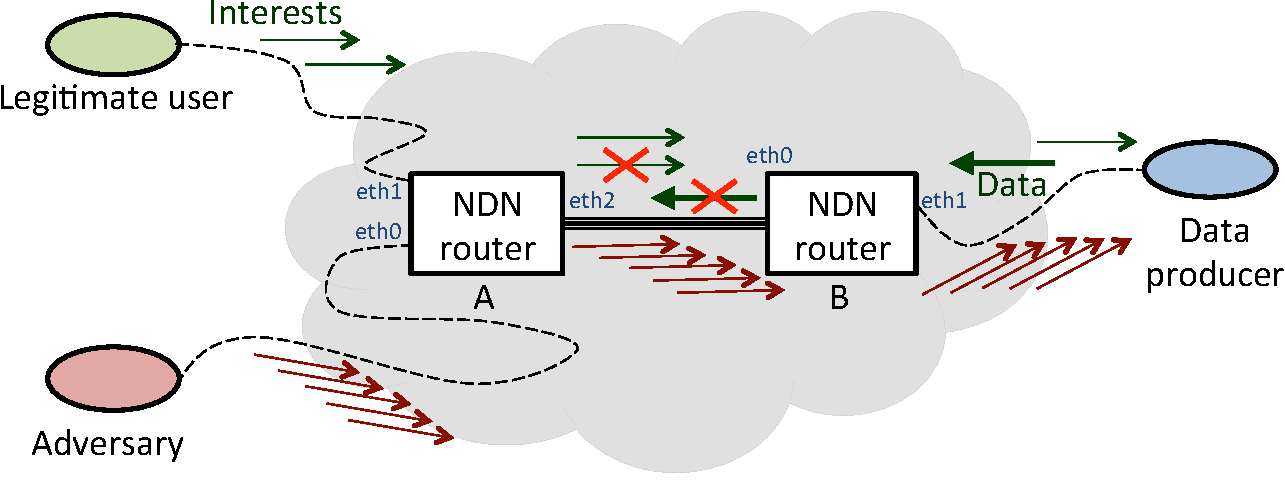
\includegraphics[scale=0.39]{attack-definition}
  \caption{Example of the Interest flooding attack}
  \label{fig:flooding example}
\end{figure}

\paragraph{How it works?}

The Interest flooding attacks can distrupt service quality in NDN network in two ways: it \emph{creates network congestion} and \emph{exhaust resources on routers}.

Like any packet in a network, Interest packets consume a portion of network capacity. Thus, Interest Flooding attacks might cause congestion and the drop of legitimate packets in the network. Although congestions might occur anywhere in the network, a coordinated DDoS attack would likely target one specific namespace to concentrate attack traffic in certain segments of the network. That is feasible for an attacker as the name prefixes loosely correspond to a network location or sets of network locations in network. 

As NDN routers maintain per-packet states for each forwarded Interest (i.e., an entry in its Pending Interests Table), an excessive volume of malicious Interests can lead to exhaustion of routers' memory. When a router has insufficient memory to create a new PIT entry, it has to drop new incoming Interests.
% there is no point in forwarding the Interest further.
% Otherwise, if Data comes back, it would be considered unsolicited and dropped anyways.
Therefore, the service for legitimate users can be disrupted due to limited memory resources in routers without saturating communication links to their limits.

%\paragraph{Target}

Because communication in NDN is content-centric, it is unlikely for an adversary to be able to target specific routers or end-hosts, as neither of them is required to have a globally routable network identity/address. However, an adversary can target a specific namespace.
For example on Fig.~\ref{fig:flooding example}, if the Data producer is the exclusive owner of \ndnName{/foo/bar} namespace and is single-homed to router B, both router B and the Data producer would receive all Interests for \ndnName{/foo/bar/\ldots} that cannot be otherwise satisfied from in-network caches. In the case of multi-homed users with rich connectivity through multiple providers, NDN would likely to cope better with DDoS attacks due its native multi-path and adaptive forwarding~\cite{adaptive-forwarding}.

% \paragraph{Countermeasures}?

%\paragraph{Effectiveness}

To efficiently implement an Interest flooding attack targeting a namespace (e.g., /newtorktimes/), an adversary needs to make sure that (1) the expressed Interests are getting as close to the Data producer as possible, and (2) the corresponding PIT entries (state) are kept on NDN routers for as long as possible.\footnote{While NDN allows users to specify lifetime of the Interest inside the Interest packet~\cite{ndn-conext,ndn-tr}, it is router's decision for how long it is willing to keep the PIT entry.  For example, and we assume this in the rest of the paper, the maximum time for which any Interest is admitted is one second.}

In order to achieve both requirements most effectively, malicious Interests should avoid collapsing (i.e, request a content that is different than existing PIT entries in the network) and cache hits (i.e., request unpopular or non-existing content). In other words, to maximize effect of an DDoS attack, each malicious Interest generated by an individual attack bot should request a non-existing content with a unique name (\emph{unique junk Interests}). In this paper, we exclusively focus on this particular attack strategy as it maximizes the damaging effect of each malicious Interest in the network and the same or similar countermeasures apply to all less-effective strains of the attack. 

In the rest of this paper, we use the general term \emph{Interest flooding attack} to refer to the above described attack and assume an attacker that is limited to controlling a botnet of end-hosts only (i.e, we assume the routers in the network and the computers in the victim domain are not compromised).

%\paragraph{Assumptions} 
%E: These are assumptions for the simulations on hand and particulary to test for the worst case scenario in many aspects. They are not the paper's assumption and in fact the paper first should be more general on describing all possibilities. Then it should explain the assumptions for the simulations and discuss why they make sense and do NOT favor positive results in some way. 

% - assumptions about attacker position
% - assumptions about the producer / producer namespace
% - assumptions about the attack traffic / attack pattern

%In this paper we are making the following assumptions about the Interest flooding attack:
%\begin{itemize}
%\item only client nodes can be compromised and become attack bots;
%\item there are no colluding attackers inside the Data producer's network;
%\item the attack is carried only using unique junk Interests; and
%\item there is only one Data producer for the attacked prefix.
%\end{itemize}

%We also assume that NDN forwarding strategy uses only single-path Interest forwarding, always choosing the best-metric route advertised by the routing protocol.
%This way, we are able to analyze the attack in its best environment, as enabling the multi-path forwarding would only alleviate effects of the Interest flooding attack.

%In section~\ref{sec:discussion} we discuss potential of the Interest flooding attack under several other attack assumptions.

%%% Local Variables: 
%%% mode: latex
%%% TeX-master: "paper"
%%% End: 
